\section{Auswertung}
\label{sec:Auswertung}

\subsection{Verifizierung der Funktionsweise eines Lock-In-Verstärkers}
\label{subsec:Verifizierung}
Die Spannungen werden für 7 Phasenverschiebungen in 60° Abständen aufgenommen.
Die entsprechenden Bilder des Oszilloskop sind in \autoref{fig:ohne} zu finden.

\begin{figure}
  \begin{subfigure}{0.48\textwidth}
      \centering
      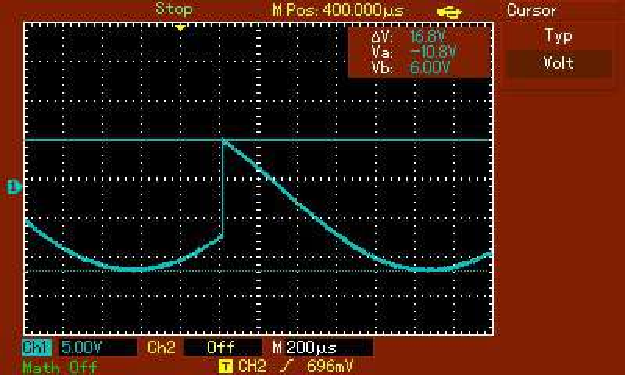
\includegraphics[height=5cm]{content/abbildungen/ohne/0.pdf}}
      \caption{Spannung bei $\phi = 0°$.}
      \label{fig:ohne_0}
  \end{subfigure}
\hfill 
  \begin{subfigure}{0.48\textwidth}
      \centering
      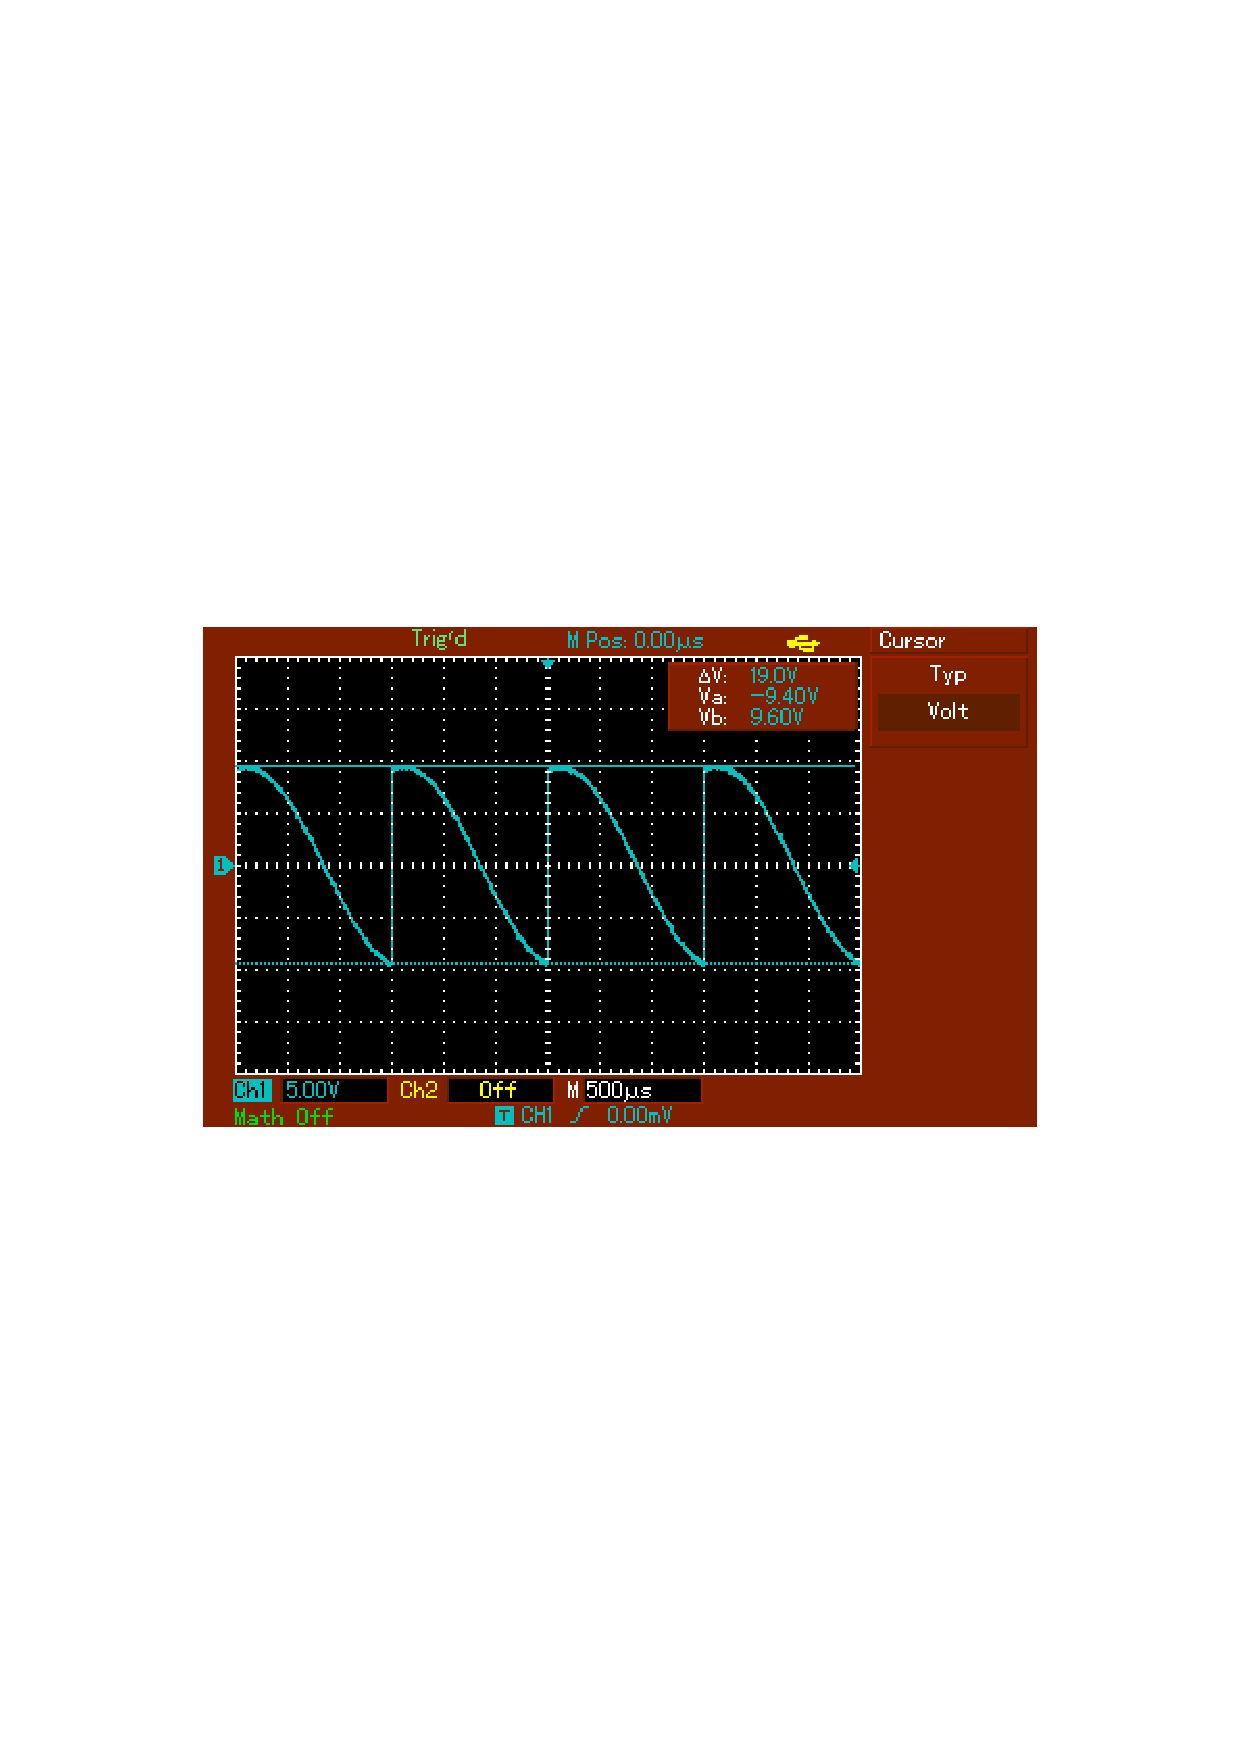
\includegraphics[height=5cm]{content/abbildungen/ohne/60.pdf}
      \caption{Spannung bei $\phi = 60°$.}
      \label{fig:ohne_60}
  \end{subfigure}
\hfill 
  \begin{subfigure}{0.48\textwidth}
      \centering
      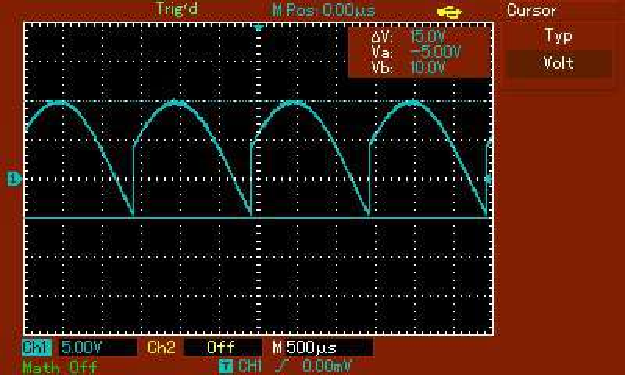
\includegraphics[height=5cm]{content/abbildungen/ohne/120.pdf}
      \caption{Spannung bei $\phi = 120°$.}
      \label{fig:ohne_120}
  \end{subfigure}
\hfill 
  \begin{subfigure}{0.48\textwidth}
      \centering
      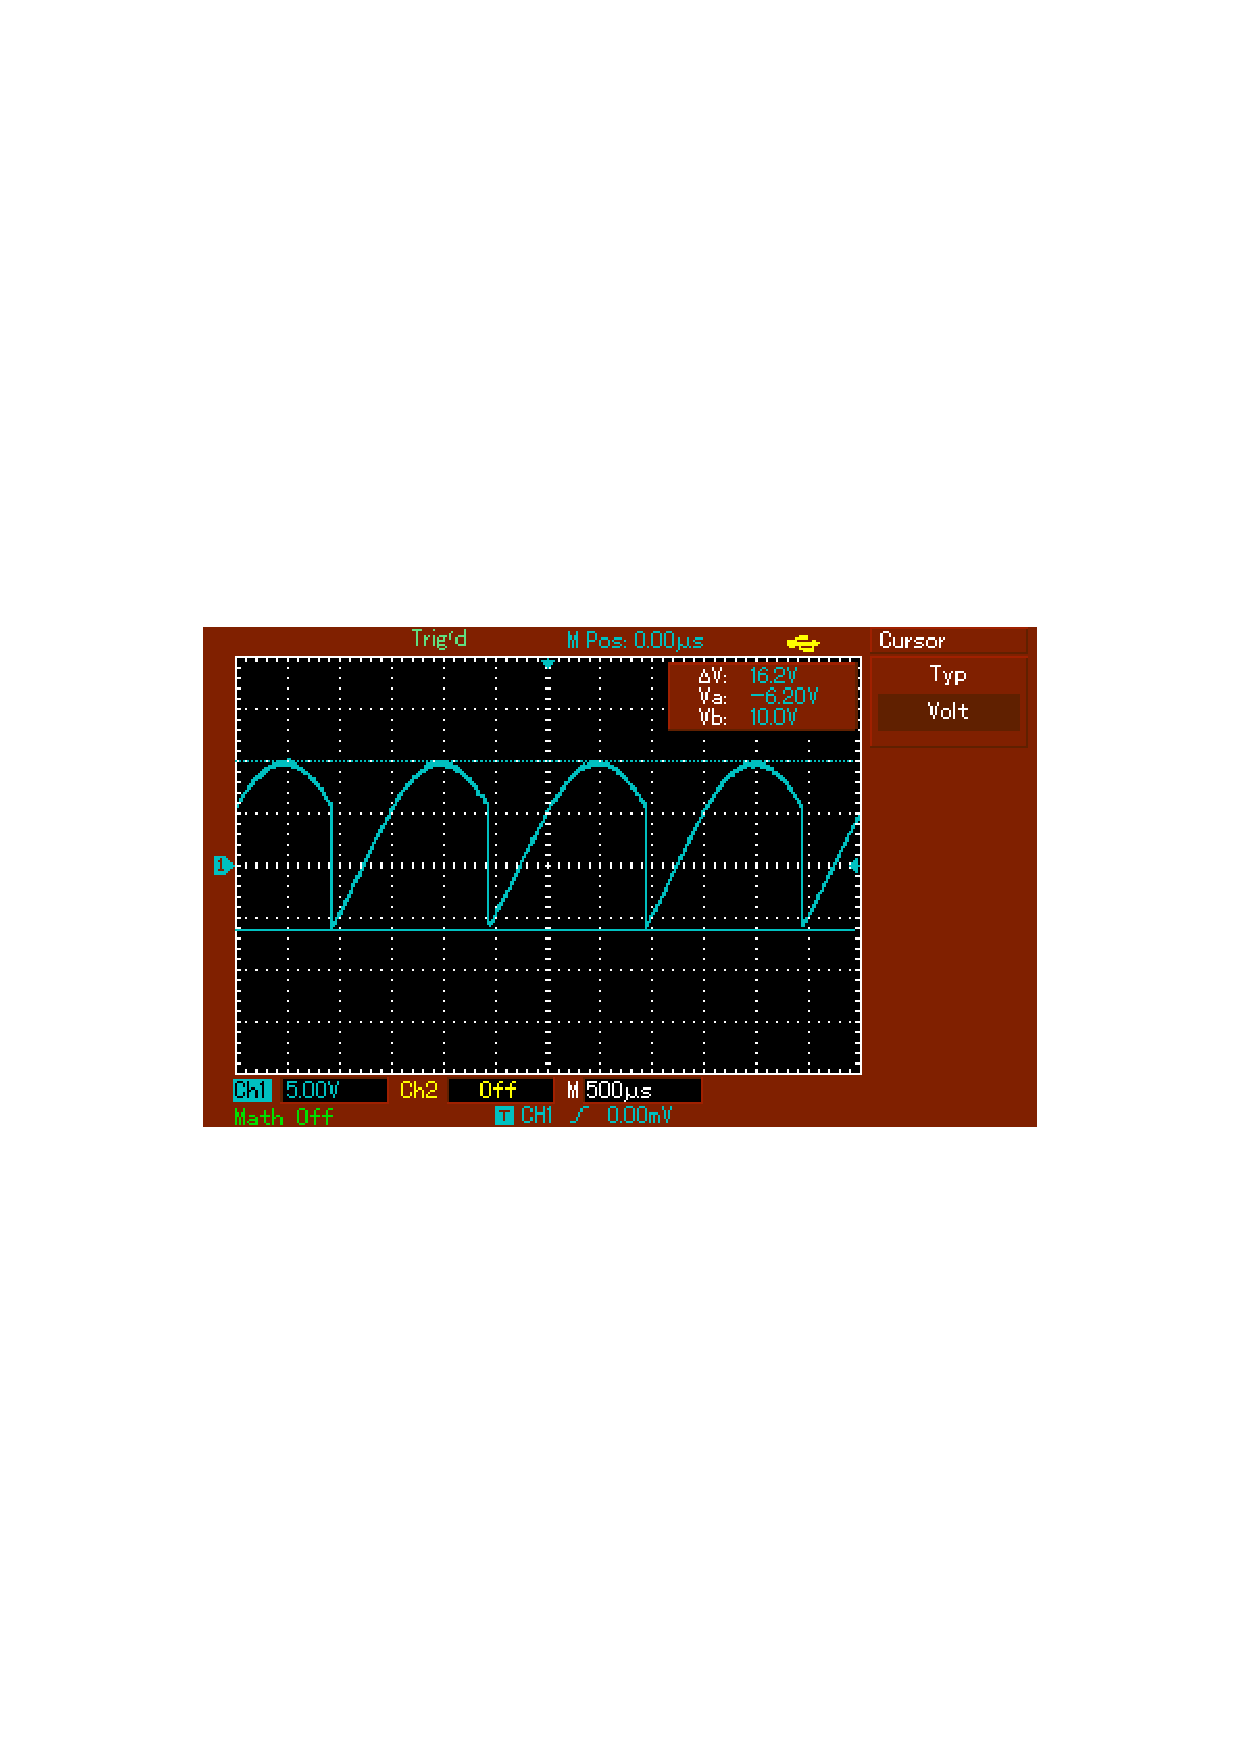
\includegraphics[height=5cm]{content/abbildungen/ohne/180.pdf}
      \caption{Spannung bei $\phi = 180°$.}
      \label{fig:ohne_180}
  \end{subfigure}
\hfill 
  \begin{subfigure}{0.48\textwidth}
      \centering
      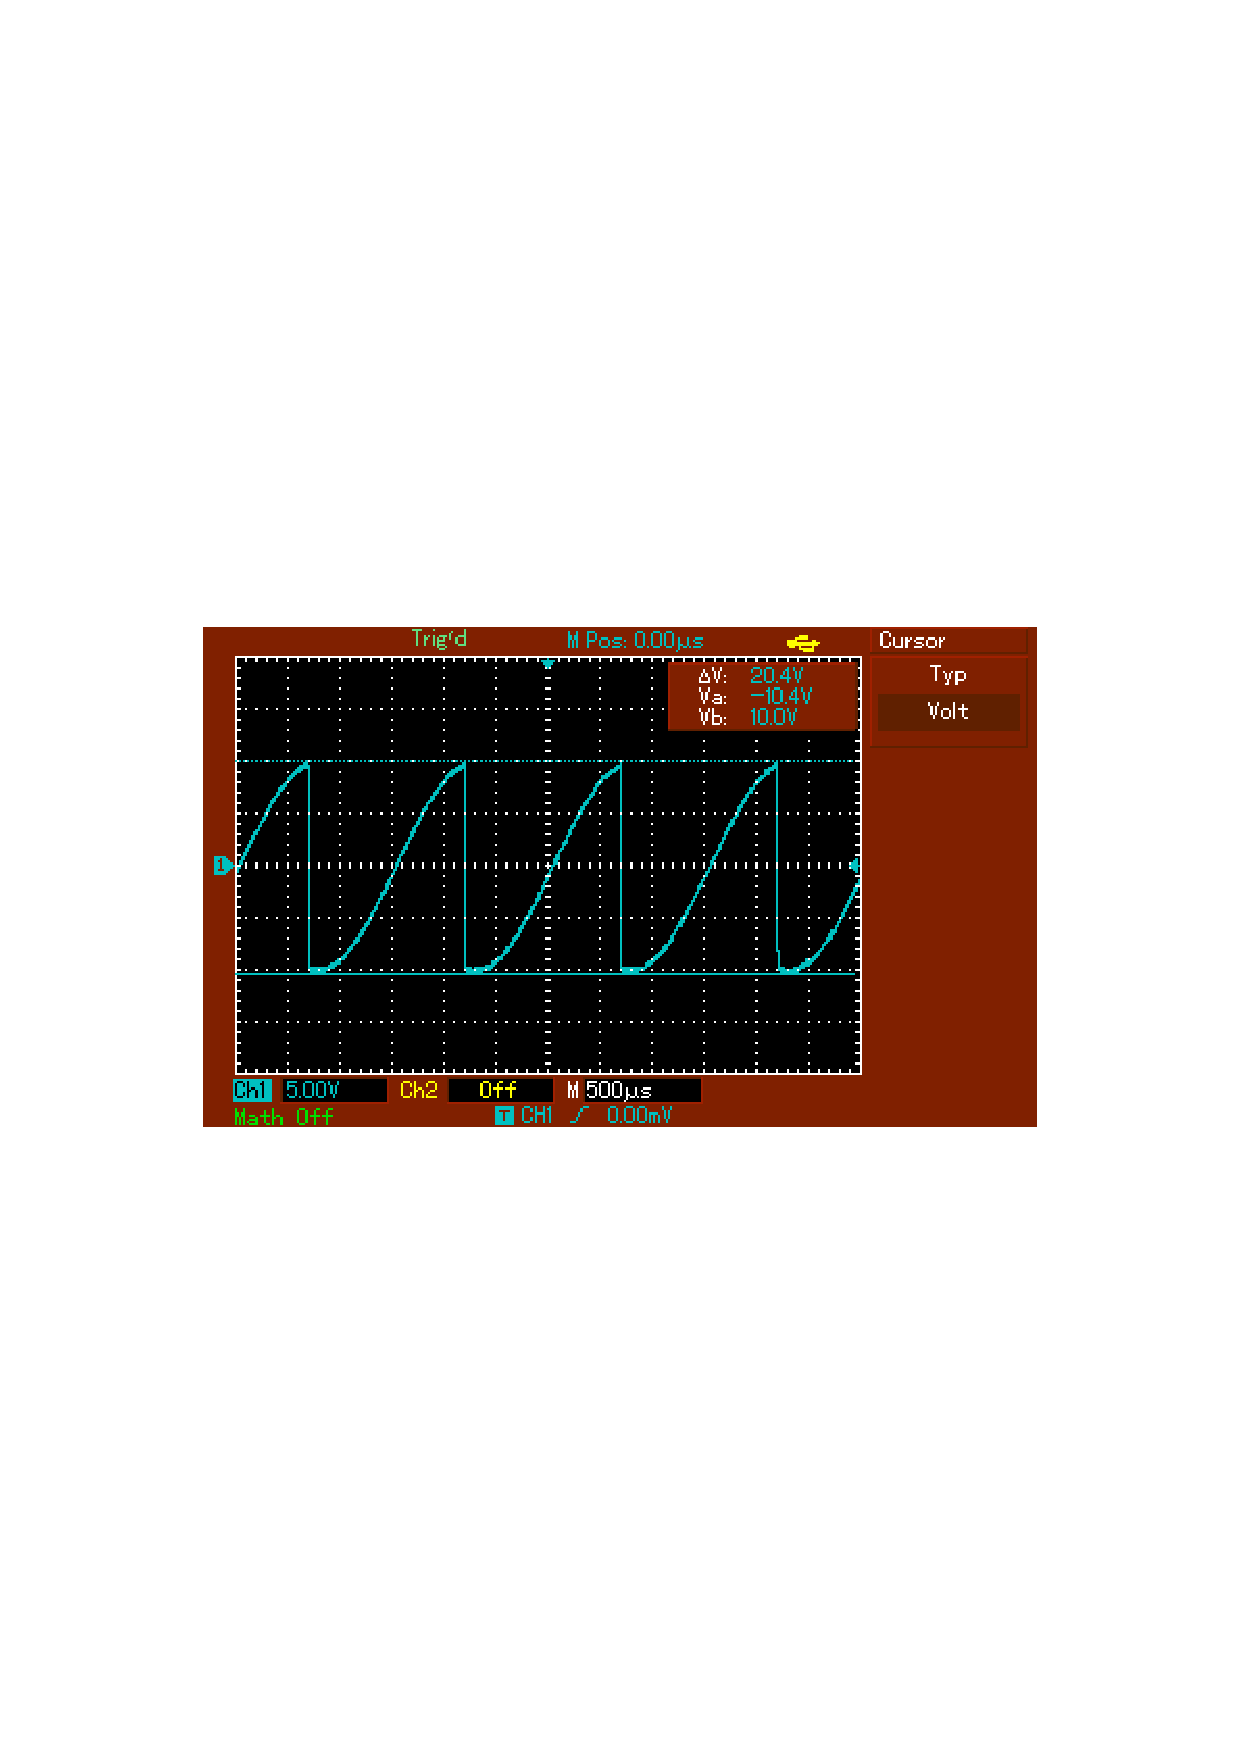
\includegraphics[height=5cm]{content/abbildungen/ohne/240.pdf}
      \caption{Spannung bei $\phi = 240°$.}
      \label{fig:ohne_240}
  \end{subfigure}
\hfill 
  \begin{subfigure}{0.48\textwidth}
      \centering
      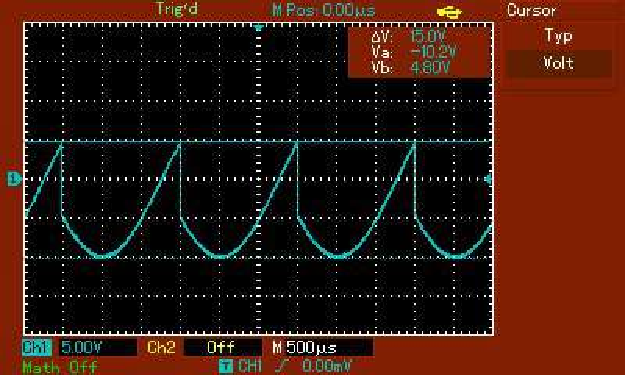
\includegraphics[height=5cm]{content/abbildungen/ohne/300.pdf}
      \caption{Spannung bei $\phi = 300°$.}
      \label{fig:ohne_300}
  \end{subfigure}
\hfill 
  \begin{subfigure}{0.48\textwidth}
      \centering
      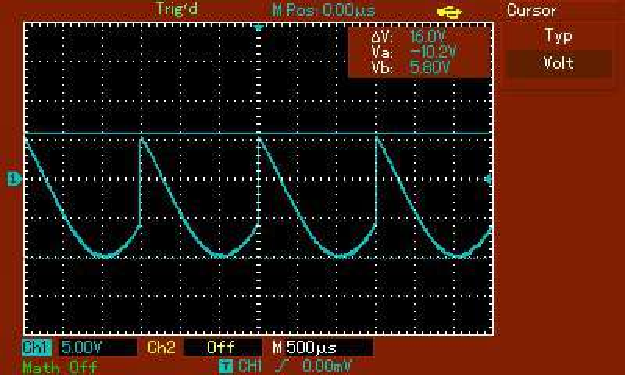
\includegraphics[height=5cm]{content/abbildungen/ohne/360.pdf}
      \caption{Spannung bei $\phi = 360°$.}
      \label{fig:ohne_360}
  \end{subfigure}
\caption{Die Spannungen bei verschiedenen Phasenverschiebungen $\phi$.}
\label{fig:ohne}
\end{figure}

\begin{table}
  \centering
  \caption{Die aufgenommenen Messergebnisse. Die Spannung in Abhängigkeit von der Phasenverschiebung $\phi$, mit und ohne Noise Generator. } 
  \label{tab:data_ohne_mit}
  \begin{tabular}{c c c}
    \toprule
    $\increment \phi /°$ & $A_\text{ohne Noise} [\si{\volt}]$ & $A_\text{mit Noise} [\si{\volt}]$ \\
    \midrule
    0    &   8.4   &  5.85  \\
    60   &   9.5   &  3.72  \\
    120  &   7.5   &  6.2   \\
    180  &   8.1   &  6.4   \\
    240  &   10.2  &  3.56  \\
    300  &   7.5   &  5.6   \\
    360  &   8     &  6.2   \\
    \bottomrule
  \end{tabular}
\end{table}

\begin{table}
  \centering
  \caption{Die aufgenommenen Messergebnisse. Die Spannung in Abhängigkeit von der r. } 
  \label{tab:data_dioden}
  \begin{tabular}{c c}
    \toprule
    $r / \si{\centimetre}$ & $A [\si{\volt}]$\\
    \midrule
    4.5    &   16.6  \\
  6.0    &   13.0  \\
  7.0    &   11.2  \\
  8.0    &   10.0  \\
  9.0    &   9.2   \\
  10.0   &   8.2   \\
  12.0   &   7.0   \\
  14.0   &   5.0   \\
  16.0   &   4.16  \\
  18.0   &   3.48  \\
  20.0   &   2.82  \\
  22.5   &   2.44  \\
  25.0   &   2.0   \\
  27.5   &   1.72  \\
  30.0   &   1.44  \\
  35.0   &   1.04  \\
  40.0   &   0.69  \\
  45.0   &   0.57  \\
  50.0   &   0.480  \\
  60.0   &   0.300  \\
  70.0   &   0.228  \\
  80.0   &   0.168  \\
  100.0  &   0.126  \\
    \bottomrule
  \end{tabular}
\end{table}
